

\documentclass{sig-alternate}

\usepackage{cite}
\usepackage{color}
\usepackage{courier}

\usepackage{tikz}
%\usepackage{listings}
\usepackage{balance} % Add this back in. Probably needed during camera ready.
\usepackage{pgfplots}
%%

\usepackage{graphicx}% http://ctan.org/pkg/graphicx




\usepackage{listings}
%\usepackage{pxfonts}
\usepackage{times}
%\usepackage{xspace}
\usepackage{booktabs}
\usepackage{fancybox}

\usepackage{multirow}
\usepackage{array}
\usepackage{tabularx}
\usepackage{url}
\urlstyle{same}
\usepackage{xcolor}


\usepackage{caption}
\usetikzlibrary{shapes,arrows}
\usetikzlibrary{patterns}
\usepackage[numbers]{natbib} % Used to fix formatting issue.
\usepackage{soul} % Needed for wrapping of highlighted text



% Define bar chart colors
%
\definecolor{bblue}{HTML}{4F81BD}
\definecolor{rred}{HTML}{C0504D}
\definecolor{ggreen}{HTML}{9BBB59}
\definecolor{ggrey}{HTML}{707070}
%\definecolor{ppurple}{HTML}{9F4C7C}

% Define flow chart styles
\tikzstyle{decision} = [diamond, draw, fill=blue!20,
    text width=15em, text badly centered, node distance=3cm, inner sep=0pt]
\tikzstyle{block} = [rectangle, draw, fill=blue!20,
    text width=15em, text centered, rounded corners, minimum height=4em]
\tikzstyle{line} = [draw, -latex']



\usetikzlibrary{shapes,arrows, positioning} % Needed for analysis diagram

\newcommand{\todo}[1]{\textcolor{cyan}{\textbf{[#1]}}}
\newcommand{\xxx}[1]{\textcolor{green}{{\it [xxx says: #1]}}}
\newcommand{\dan}[1]{\textcolor{blue}{{\it [Dan says: #1]}}}


\begin{document}

%\conferenceinfo{ICSE}{'2014 Hyderabad, India}

\title{A Largescale Analysis of Android Applications}

\numberofauthors{2} %  in this sample file, there are a *total*
% of EIGHT authors. SIX appear on the 'first-page' (for formatting
% reasons) and the remaining two appear in the \additionalauthors section.
%
\author{
% You can go ahead and credit any number of authors here,
% e.g. one 'row of three' or two rows (consisting of one row of three
% and a second row of one, two or three).
%
% The command \alignauthor (no curly braces needed) should
% precede each author name, affiliation/snail-mail address and
% e-mail address. Additionally, tag each line of
% affiliation/address with \affaddr, and tag the
% e-mail address with \email.
%
% 1st. author
\alignauthor
Daniel E. Krutz and xxxx\\
       \affaddr{Affiliation}\\
       \affaddr{xxx1 Lomb Memorial Drivexxx}\\
       \affaddr{xxxRocheser, NY, USAxxx}\\
       \email{\{xxxxdxkvse, xxxx\}@rit.eduxxxx}
}
% 2nd. author
%\alignauthor
%G.K.M. Tobin\titlenote{The secretary disavows
%any knowledge of this author's actions.}\\
 %      \affaddr{Institute for Clarity in Documentation}\\
  %     \affaddr{P.O. Box 1212}\\
  %     \affaddr{Dublin, Ohio 43017-6221}\\
   %    \email{webmaster@marysville-ohio.com}


\maketitle
\begin{abstract}

Abstract

- What the problem is
- What our research is
- What were some of our initial findings
-




\end{abstract}

\todo{Update these}
% A category with the (minimum) three required fields
\category{H.4}{Information Systems Applications}{Miscellaneous}
%A category including the fourth, optional field follows...
\category{D.2.8}{Software Engineering}{Metrics}[complexity measures, performance measures]

\terms{}

\keywords{xxxxxxxx}

\section{Introduction}

% Use stats from http://www.androlib.com/appstats.aspx
There are over 675,000 Android applications with over 12,000 being added every month. \todo{find citations and update values}. Mobile applications (apps) are typically updated more frequently than traditional desktop applications\todo{cite}, with many apps being updated several times a month. These updates occur for a variety of reasons including bug fixes, required updates for new phone hardware, or feature additions. While the intention is for each release is to make the software better, unfortunately they often cause more harm than good. These range from minor coding issues and maintenance difficulties for the development team, to significant security vulnerabilities which may expose the user to serious malicious actions. Additionally, when the end user installs an updated versions of an app, they typically believe that they are getting an enhanced version of the software, whether it be from the security, stability or functionality perspective.

The goal of this research is to understand how Android apps evolve over time from the perspective of security vulnerabilities, defects, maintainability, adherence to coding standards, and application size.\dan{We are collecting much data, should we list it all?}  Specifically, we will address the following research questions:

\textbf{RQ1:}~\emph{How did the security vulnerability of Android applications change over time}\\
Did apps generally become more secure over time? How did the permissions gap evolve over time, and what were some of the common over and under privileges which occurred?


\textbf{RQ2:}~\emph{How do apps compare against known malware?}\\
How do the ratings of applications which are not known to be malicious compare against applications which are know to be malicious in a variety of metics \dan{This really needs to be reworded}

\textbf{RQ3:}~\emph{Can defect count and other metrics predict the number of downloads and user ratings for the~\emph{current} release of an app?}\\

% Download count will need to be somehow normalized over the number of months an application was available. This cannot be done by simply averaging the number of months since I will guess that more applications are downloaded when an application initially arrives.
% Download count could also be a problem since we will be getting the number of downloads when an application is first released.


\textbf{RQ4:}~\emph{Can poor coding standards and clones predict metrics about~\emph{future} releases of an app?}\\
Can the use of poor coding standards predict that future releases of an application will contain more defects. Also, can they predict the user ratings \& number of downloads for the future releases of the app?


\textbf{RQ5:}~\emph{What correlations exist between metrics such as defects, coding standards and code clones with the vulnerability of the software?}\\
Blah Blah blah


%\textbf{RQ2:}~\emph{Question?????}\\
%Blah Blah blah




%\textbf{RQ2:}~\emph{Question?????}\\
%Blah Blah blah

%%%%%%%
%\textbf{RQX:}~\emph{Question?????}\\
%Blah Blah blah
%%%%%%%


\dan{This will need to be tweaked, these are just some I am starting with}

\todo{Modify the format of this}
This work is important because  \dan{really work on this}

\begin{itemize}
  \item Provide insight on the lifecycle of mobile applications - Can help improve how apps are written in the future. What types of correlations occur
  \item Provide insight if newer applications are generally better
  \item Provide a data set for future developers and researchers
\end{itemize}

The contributions of this paper are:



The rest of the paper is organized as follows. Section~\ref{sec: oraclecreation}

\label{sec: androidapplications}
\section{Android Applications}

The Android operating system has emerged as a market leader in mobile computing, comprising over \todo{xxx} of the mobile market.


\subsection{Android Application Structure}

The Android application stack is comprised of four primary layers. The top layer is the Android application layer, which is followed by the the three application framework layers. The Android Software Development Kit (SDK) allows developers to create Android applications using the Java programming language.

Isolation between Android applications is enforced through the use of the Android sandbox~\footnote{http://developer.android.com/training/articles/security-tips.html}, which prevents applications from intruding upon one another. Application developers are required to explicitly declare the required application permissions in the~\emph{AndroidManifest.xml} file. This will allow the application to request privileges to specific functionality such as the ability to write to the calendar, or access the GPS. Before installing the application, the user is asked to accept or reject these requested permissions. Once installed, the developer cannot remotely modify the permissions without releasing a new version of the application~\cite{shaerpour2013trends}. This differs from iOS \todo{- How does this differ from iOS}


\emph{Intents} are a communication mechanism which use~\emph{Activitys} to exchange information between the components of an Android application. Inter Process Communication (IPC) is the composition mechanism performed using intents which is used to invoke another application component. There are three types of attacks which exploit Intents for malicious reasons. These include~\emph{permission collusion},~\emph{confused deputy} and~\emph{Intent Spoofing}~\cite{6641043}.\todo{Add to this}



An Android Application Package File(apk) contains all of the files necessary to install an Android application and is essentially just a compressed file of the application's source code. There are several key components of an apk file, which are shown in Table~\ref{Table:apkcontents}.


%% Much of this able came from : ~\cite{Lee_2013}
\begin{center}

\begin{table}[ht]% Try here, and then top
\caption{APK Contents}
\label{Table:apkcontents}
  \begin{tabular}{ l | l  }

    \bfseries File & \bfseries Description \\ \hline
    AndroidManifest.xml & Permissions \& app information \\ \hline
    Classes.dex & Binary Execution File \\ \hline
    /res & Directory of resource files \\ \hline
    /lib & Directory of compiled code \\ \hline
    /META-INF & Application Certification \\ \hline
    resources.arsc & Compiled resource file \\
  \end{tabular}
\end{table}
\end{center}


Android applications may be released to the user in a variety of methods, with the most popular being through the GooglePlay store\footnote{https://play.google.com/store}, while many are downloaded through alternative sites such as AppksAPK\footnote{http://www.appsapk.com/} and F-Droid\footnote{https://f-droid.org/}. This differs from iOS applications which are all forced to go through an Apple controlled central App Store. While the exact steps taken by Apple to ensure the quality of their applications is unknown, it is believed that they do check all apps submitted to the app store for various security standards~\cite{Chin:2012:MUC:2335356.2335358}. Android users enjoy more freedom to download from a wider range of sources however, they are not provided with any of the verification which the Apple App Store states to provided.

- What are some problems seen?

\subsection{Android Permission Structure}
\dan{cut this down a bit?}
The Android security model is a permission-based system where applications need to be granted access to various areas of functionality before they may be used. If an application attempts to perform an operation which it does not have permission, a~\emph{SecurityException} is thrown. When an Android application is created, its developer must declare in advance what permissions the application will require~\cite{Felt:2011:APD:2046707.2046779}. These security settings are stored in the~\texttt{AndroidManifest.xml} \todo{redundant} file and include a ride range of permissions including the ability to transmit data, access personal information, and charge subscription fees~\cite{Barrera:2010:MEA:1866307.1866317}. A few of these are~\emph{INTERNET},~\emph{READ\_CONTACTS}, and ~\emph{WRITE\_SETTINGS}. When an application is invoked, this manifest file is examined to determine the appropriate permissions the application should possess.

A basic principle of software security is the~\emph{principle of least privilege}, or the granting of the minimum number of privileges that an application needs to properly function~\cite{saltzer1975protection}. Granting more privileges than the application actually needs creates security problems since vulnerabilities in other applications, or malware, could use these extra permissions for malicious reasons. Additionally, this limits potential issues due to non-malicious, developer errors.

Unfortunately, developers are often forced to grant more permissions to their application than they actually need. Due to the granularity of the permission spectrum used by Android, the developer must often grant more permissions to their application than it actually requires. For example, an application which needs to send information to one site on the Internet will need to be given full permissions to the Internet, meaning that it may communicate with with all websites~\cite{jeon2011dr}.

Each Android permission is assigned under one of several protection levels which helps to define the risk level associate with each permission~\cite{permissionLevelsURL}. These levels are:

\begin{description}
  \item[Normal] Default value with minimal risk. Grants the application access to isolated, application level features. Minimal risk is incurred by other applications and the end user.
  \item[Dangerous] An elevated permission risk which provides the application access to private user information or control over the device should could negatively impact the end user. Upon the instillation of an application, the user needs to explicitly grant these permissions.
\item[Signature] Highest level of permission. Granted by the system only if the application is signed by the same certificate as was declared in the permission. The user is not notified that this permission is granted if the certificates match, and the application will automatically possess these privileges.
  \item[signatureOrSystem] Application must be in the Android system image or signed with the same certificate as the application which declared the permission. The majority of developers should avoid using this protection level, as it was intended for use by applications created by multiple vendors who needs to have them built into the system image.

\end{description}


The number of Android permissions has risen from 103 in API Level 3 (Cupcake), in 2009 to over xxx in API 19 (KITKAT)\todo{find number and citation}. This list is expected to continue to grow, with the permissions in the~\emph{Dangerous} group the largest, and fastest growing. Permissions are added over time as device functionality grows and changes~\cite{Wei:2012:PEA:2420950.2420956}.


- What are some ways that permissions are mis-used?



%% A good resource for this section is
%%28-2
%%8-4
%%29-3.2
%%30-2.2
%%2-2A
%%10-2.3
%% Functionality categories 10



\label{sec: dca}
\section{Data Collection \& Analysis}

We analyzed over xxxx\todo{update number} Android application files over a period of xxxx \todo{update} using a variety of different tools. The results were stored in a publicly accessible database located on our project website. \todo{Add link to website}

\label{sec: collection}
\subsection{Collection Process}

The Android apk files were pulled from GooglePlay using a custom built collector using~\emph{Scrapy}~\cite{scrapy_URL} as a foundation. We chose to pull from GooglePlay since it is the most popular source of Android applications and was able to provide various application information such as the developer, version, genre, number of downloads, user rating and number of downloads. Our scraper was initially run to randomly collect~\todo{xxxx} apk files, which were then decompiled and further analyzed. 

\subsection{Decompliation}
\label{sec: decompliation}

The downloaded .apk files had to be decompiled to .class and .java files to be further analyzed. The first step was to unzip the .apk file using a simple unix command. However, two open source tools were required to complete the decompilation process. These were:
 \begin{description}
    \item~\textbf{dex2jar:} Converts the .dex file into a .jar file. A java jar command is then used to convert this to .class files~\cite{dex2jar_key}.
    \item~\textbf{jd-cmd:} A command line decompliler which converts .class files to .java~\cite{jdcmd_key}.
\end{description}

The number of extracted class and java files are recorded. The de-compilation process is shown in Figure~\ref{fig:extractionprocess}.

\begin{center}

%\label{fig:extractionprocess}

% ~\cite{Lee_2013} %% This diagram is largely copied from here

% Define block styles
\tikzstyle{line} = [draw, -latex']
\tikzstyle{cloud} = [draw, ellipse,fill=white!20, node distance=2.2cm,
    minimum height=2em]
\begin{figure}[h]
\caption{APK Extraction Process}
\label{fig:extractionprocess}
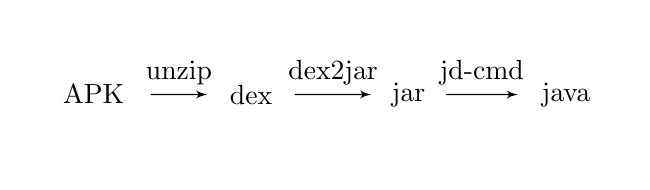
\begin{tikzpicture}[node distance = 2cm, auto]
    % Place nodes
     \node [cloud] (init) {APK};
     \node [cloud, right of=init] (dex) {dex};
     \node [cloud, right of=dex] (jar) {jar};
     \node [cloud, right of=jar] (java) {java};

     \path [line] (init) -- node {unzip}(dex);
     \path [line] (dex) -- node {dex2jar}(jar);
     \path [line] (jar) -- node {jd-cmd}(java);

\end{tikzpicture}
\end{figure}
\end{center}

\subsection{Analysis Process}
\label{sec: analysis}

The next phase was to analyze the extracted source code for a variety of metrics in order to more appropriately understand how they evolve. Some of which included the vulnerability of the application from a security perspective, permissions gap, detected bugs, misuse of coding standards and software clones. These are functionally equivalent portions of an application which may differ syntactically and are often a sign of poorly written software and may be detrimental to an application in a variety of ways. Some of which include increased maintenance costs since changes will need to be done several times and inconsistent bug fixes~\cite{Roy:2009:CEC:1530898.1531101}.

This analysis was accomplished using a variety of existing tools including:

 \begin{description}
    \item~\textbf{Stowaway\cite{Felt:2011:APD:2046707.2046779}:}Reports the overpermissions and underpermissions of an application. We recorded the overpermissions of the application, as well as all areas the application was underprivledged.
    \item~\textbf{AndroRisk\cite{androguard_url}:}A component of the Androguard reverse engineering tool, this tool reports the risk indicator of an application for potential malware. We recorded the report risk level for the apk file.
    \item~\textbf{CheckStyle\cite{checkstyle_key}:}A developent tool to measure how well developers adhere to coding standards. Some of which include naming conventions, annotation usage, size violations and empty block checks. We recorded the total number of violations of these standards. Default values were used in our analysis.
    \item~\textbf{Jlint\cite{jlint_key}:} Examines java code to find bugs, inconsistences and synchronization problems by conducting a data flow analysis and building lock graphs. We recorded the total number discovered bugs. This tool was selected over FindBugs~\cite{findbugs_key} since it was able to analyze the applications much faster. \todo{say something about findbugs??}
    \item~\textbf{Simcad\cite{6613857}:} A powerful software clone detection tool. This tool was selected over other clone detection tools such as Nicad~\cite{Cordy:2011:NCD:2057176.2057234}, CCCD~\cite{6671332} and MeCC~\cite{Kim:2011:MMC:1985793.1985835} due to its ability to quickly detect a wide variety of clones. We recorded the number of clones discovered by Simcad for each target application.
    \item~\textbf{APKParser~\cite{apkparser_link}:} A tool to read various information from an Android apk file including the version, intents, and permissions. We used the output from this tool to determine the application version, minimum sdk, target sdk, required intents, and requested permissions.



\end{description}


\todo{Make sure to provide good justification for the use of selected tools. IE why was one tool chosen over another...}

% Why JLint was used http://www.cs.umd.edu/~jfoster/papers/issre04.pdf
%%% Good resource with statistics of jlint vs findbugs

Stowaway and Androrisk were able to analyze the raw apk files. CheckStyle, Jlint and Nicad required the apk files to be decompiled. All results were recorded in a sqliteDB, which is publicly available on the project website. The full analysis process is shown in Figure~\ref{fig:analysisprocess}.

\begin{figure}[h]
\begin{center}
\caption{APK Analysis Process}
\label{fig:analysisprocess}
% Define block styles
\tikzstyle{line} = [draw, -latex']
\tikzstyle{cloud} = [draw, ellipse,fill=white!20, node distance=2.2cm,
    minimum height=2em]
\tikzstyle{block} = [rectangle, draw, fill=white!20,
    text width=5em, text centered, rounded corners, minimum height=4em]

\tikzstyle{c} = [draw, cylinder, shape border rotate=90, aspect=0.75, %
      minimum height=70, minimum width=30]

\begin{tikzpicture}[node distance = 1.5cm, auto]

    % Place nodes
     \node [cloud] (init) {APK Collection};
     \node [block, below of=init] (ApkFiles) {ApkFiles};
     \node [cloud, below of=ApkFiles] (Decompile) {Decompile};
     \node [block, below of=Decompile] (DecompiledFiles) {Decompiled Files};
     \node [cloud, below of=DecompiledFiles] (JavaAnalysis) {Java Analysis};
    % \node [cloud, right of=ApkFiles] (apkanalysis) {Stowaway AndroRisk};
    % \node [c, right of=DecompiledFiles] (SqliteDB) {SqliteDB};
     \node[c] (SqliteDB) [below right=-1.0cm and 2.4cm of DecompiledFiles]
       {SqliteDB};

    \node[cloud] (apkanalysis) [below right=-0.9cm and 2.0cm of ApkFiles]
       {APK Analysis};

    % Draw edges
    \path [line] (init) -- (ApkFiles);
    \path [line] (ApkFiles) -- (Decompile);
    \path [line] (Decompile) -- (DecompiledFiles);
    \path [line] (DecompiledFiles) -- (JavaAnalysis);
    \path [line] (JavaAnalysis) -- (SqliteDB);
    \path [line] (Decompile) -- (SqliteDB);
    \path [line] (ApkFiles) -- (apkanalysis);
    \path [line] (apkanalysis) -- (SqliteDB);

\end{tikzpicture}
\end{center}
\end{figure}


\todo{Other items recorded}
- Lines of code
- Java files
- Class files
- APK FileSize
- APKParser
-   Version
-   MinSDK
-   Interprocess communications
-

\label{sec: evaluation}
\section{Evaluation}

Blah
% Clearly outline all steps and make sure that everything is repeatable.
% Show a chart of how the data changes over time.


- Discuss results
- How long did we let the scanner run
- Implications
- Interesting findings
- Answer research questions
- What are our main findings?
- Break the privileges down into threat levels (see pg 3)\cite{Felt:2011:EAP:2002168.2002175}


- Which over and under privs ocurred most often
- How many apps were over and under privs




\subsection{Comparison to Malware}

\dan{This section will need to be cleaned up}
\todo{Make sure all values are up to date}

We next compared our findings against 139\todo{update?} malware examples from the Contagio Mobile Mini Dump~\cite{contagio_url} and the Malware Genome Project~\cite{Zhou:2012:DAM:2310656.2310710} for the purpose of examining the differences between malicious and benign Android applications. Since many of the malware examples represented only slight alterations from their counterparts, one result from each malware family was taken from the Malware Genome project to help limit the negative impact that familes with many examples would have in skewing the results.

The compared areas included the adherence to coding standards, discovered defects, permission gap and the utilized intents \& permissions. This was accomplished by running the malicious applications through the same process as the benign application, as was described in Sections~\ref{sec: decompliation} and~\ref{sec: analysis}. The results of this analysis are available in our public GitHub repository. Since we were unable to unable to analyze the lifecycle of the malware examples, we took the average values for the first 10,000\dan{update} collected benign Android applications and compared them to the average values for the malicious applications. The number number of defects found by jLint and coding standards mistakes were divided by the number of classes to help normalize these results by the size of the application. The results are shown in Table~\ref{Table:maliciousvsnonmalicious}.


We found that malicious applications had a much higher number of coding standards mistakes per class compared to their benign counterparts while also having a slightly higher number of defects per class. \todo{What this means}


Not surprisingly, the malicious applications had an average of more than twice the number of over privileges as compared to their counterparts.

\dan{What are most of the over privileges}
\todo{What this means}


\begin{center}

\begin{table}[ht]
\caption{Malware vs. Non-Malicous}
\label{Table:maliciousvsnonmalicious}
  \begin{tabular}{ l | l | l }

     \bfseries Test  & \bfseries Malicious & \bfseries Regular \\ \hline
    Fuzzy Risk & 46.25 & 53.72 \\ \hline
    JLint/Class & .395 & .301 \\ \hline
    Defect Count/Class & 11.07 & 1.87 \\ \hline
    Overpriviledges & 3.3 & 1.34 \\ \hline
    Underpriviedges & 1.07 & 1.96 \\ \hline
    Intent Count & 2.05 & 2.58 \\
  \end{tabular}
\end{table}
\end{center}

%%% I do not want the values to be way off from the overall totals since
\todo{Make sure to compare this to the overall averages of all "regular" applications}
\todo{For the genome project, break each set of malware into seperate groups. This is because each group is a family of malware, and using all and aggregating the data could create problems}

% Compare the stats of these applications

% ? Show a bar chart of the aggregate malware data vs. non-malware
% Discuss the results


We next compared fake, malicious copies of Netflix and Player as identified by the Malware Genome Project. A single fake copy of Netflix was included, with six fake copies of Player. We ran these fake copies of the applications against legitimate versions attained from the GooglePlay store. In both instances, the fake versions of the applications were significantly smaller than their real counterparts. We chose to only report on the Fuzzy Risk, over privledge count, and number of Java files since many of the other results of the analysis were not deemed useful due to the small size of the fake applications. The Fuzzy risk value was similar for both versions of the Netflix applications, but the real version of the Player application had a significantly higher value than its fake counterpart. The number of overprivliledges was much higher for the Fake Netflix application compared




- How did Netflix compare?
Fake = 9 over priv = total 10
Real = 2 over priv = total = 14


Fake wanted Dump, inject events, read logs, read phone state. It did not request likely none malicious actions such as vibrate, expand status bar and system\_alert\_window

See pg 75 in "Contrasting Permission Patterns beteen Clean and Malcious Android applications"


- Look at where things are over privileged

Full results are shown in Table~\ref{Table:fakesvsRegular}.



\begin{center}

\begin{table}[ht]
\caption{Fakes vs. Regular}
\label{Table:fakesvsRegular}
  \begin{tabular}{ l | l | l | l }

    \bfseries Application  & \bfseries Fuzzy Risk  & \bfseries Over Privileges & \bfseries Java Files \\ \hline
    Fake Netflix & 51 & 9 & 11 \\ \hline
    Netflix & 50 & 2 & 2429 \\ \hline \hline
    Fake Player (Avg) & 50 & 0 & 14 \\ \hline
    Player & 92 & 0 & 813 \\ 
  \end{tabular}
\end{table}
\end{center}




- Fakes are smaller
- No discernable difference in Fuzzy Risk


- What were the fakes?



- ******** Separated by each Genre
% Good helper site
% http://nces.ed.gov/nceskids/createagraph/default.aspx?ID=b9165d963f354265ad361e09bc98eb05

- Correlations for jLint \& ratings
-		At least 10,000 downloads \& 5 apps
-	People cared more about ratings for business, Communication, Personalization, productivity
-	No affect for games, Entertainment,  Music and Audio, 
- 	Inversely proportional for lifestyle, 


\subsection{Effects of Genre}
Blah Blah Blah

\subsection{Overused Permissions}


A basic principle of security is the granting of the least amount of privileges to an application which it needs to properly function. Granting extra privileges creates unnecessary security vulnerabilities \dan{cite}. We analyzed the most overused permissions in  41 application genres ranging from communication and productivity, to sports, puzzles and entertainment. In 12 of the genres, the most over used permission was~\emph{android.permission.GET\_ACCOUNTS}, which permits access to the list of accounts in the accounts service~\cite{manifest_url}. This was followed by~\emph{android.permission.CALL\_PHONE} which allows an application to start a phone call without the user confirming it through the dialer interface. Both of which are on the API level 1 interface

\todo{Talk about why they are dangerous}

In Table XXX, we show the 



- Show table of results




\subsection{Defects \& User Ratings}
- How to defects affect ratings

- User ratings go up when a file is downloaded more (not surprsing), was very slight.
- Less coding standards issues for apps which were downloaded more



\subsection{Application Lifecyle}

%- How does quality change across genres
%- 	Which items are overpriviledged more often?
%-  	Affect of development lifecyle
%- 


We examined the effect the version of the application had on the observed quality and user rating for the application. All applications downloaded from GooglePlay were grouped together according to their application version. We separated all applications into nine distinct groups based on their version, where applications with a version number of 0 - .99 being assigned to group 0, applications with the version of 1 - 1.99 went to group 1 and so on. Based on our collected applications, there was a need of 8 groups, with 342 applications not being unable to be grouped, and were therefore ignored in this analysis. We then averaged the already determined scores for the groups to determine their average fuzzRisk, number of over-permissions,  discovered defects, and adherence to coding standards. Adherence to coding standards was determined by dividing the number of mistakes found for each application, by the number of classes in it, with the same process being used to determine defects. FuzzRisk, code clones and over permissions were found by finding the average values of each for all applications in each group. User ratings were not considered since they were virtually identical, ranging from 3.9 - 4.2. Finally, to assist with the visual representation of the results, values were normalized in the chart to follow consistent values with one another, while retaining their accuracy \todo{reword}. The results are shown in shown in Figure~\ref{VersionEffect}, with further data provided on our project webpage.

Some of our findings are:

\textbf{Applications become less secure over time}: Not only did the FuzzRisk grow over each version, but the number of over-permissions generally grew as well. This indicates that as applications evolve, they become less secure and that developers are not using proper security standards and are not checking for over permissions. While each of these values grew, there is not a direct correlation between them.


\textbf{Fuzz Risk \& Coding Standards are inversely related}:  The fuzz risk for each application version progressively became larger from version group 0 to version group 6, with a slight drop off for the version 7 group while the adherence to coding standards progressively became better, until there was a slight rise in group \#7. There does not appear to be a strong correlation between adherence to coding standards and the number of application over-permissions. \dan{talk about why this is important?}


\textbf{Over time, developers pay more attention to general quality than security}: The number of discovered clone clones, number of class files, and discovered of an application generally decrease as the application becomes more mature. This indicates that developers are refactoring and eliminating issues during the application's life cycle. Unfortunately, it does not appear as though they paying enough attention to security vulnerabilities in the application. 

% - Defects and coding standards are related
-% Overpermission rate is not related to anything
%- Talk about what you would expect in application development. 


\begin{figure*}
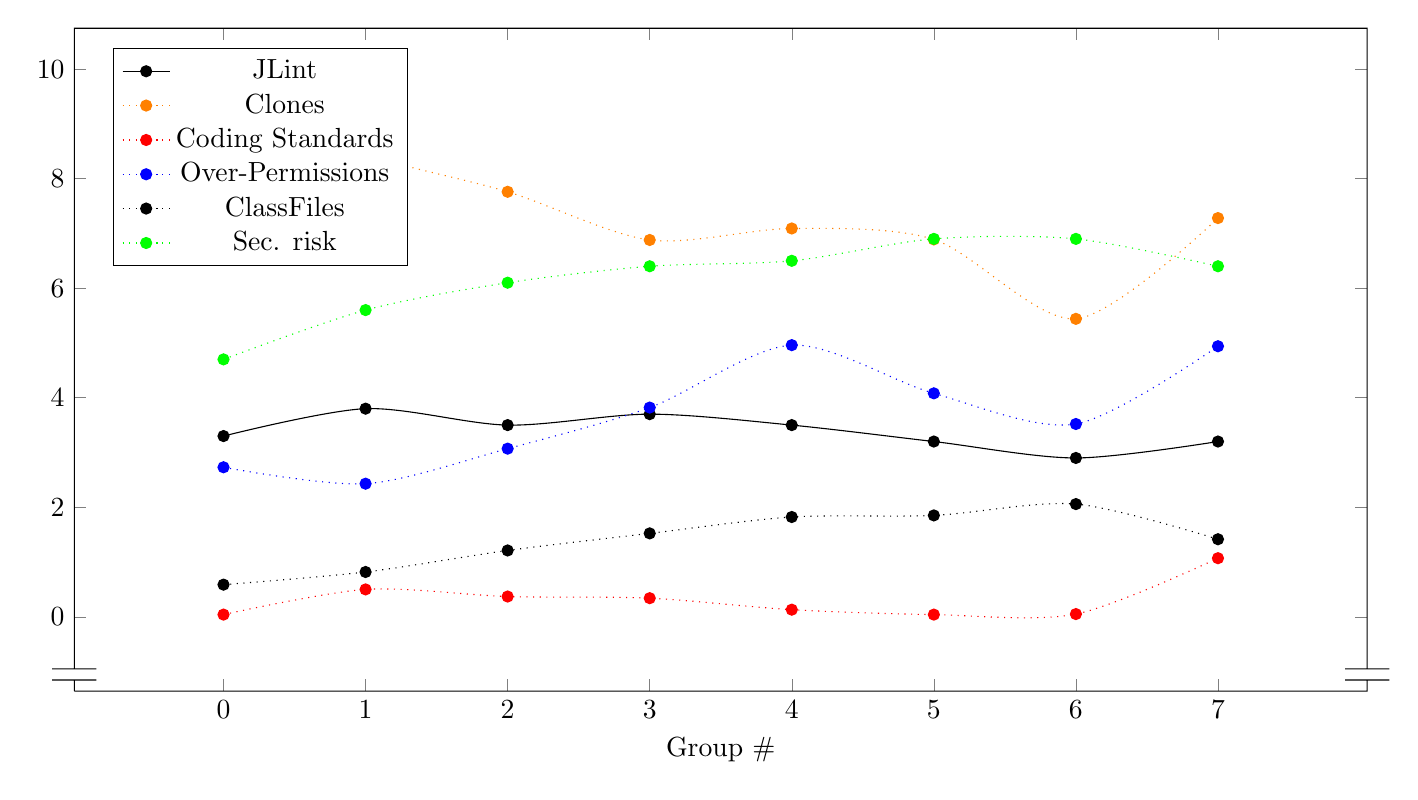
\begin{tikzpicture}
\begin{axis}[
   smooth,
   width=18cm,
   height=10cm,
   enlargelimits=0.15,
	xlabel={Group \#},
 %  ylabel={Values},
  symbolic x coords={0, 1, 2, 3, 4, 5, 6,7},
 xtick=data,
  x tick label style={rotate=0,anchor=north},
  legend pos=north west,
 axis y discontinuity=parallel,
  ]	

\todo{Update data}


% Defects - jLint
\addplot+[color=black,black,mark=*,mark options={solid},smooth] plot coordinates {(0,3.3) (1,3.8) (2,3.5) (3,3.7) (4,3.5) (5,3.2)(6,2.9)(7,3.2)};
\addlegendentry{JLint}


% Clones
\addplot [color=orange,dotted,mark=*,mark options={solid},smooth] plot coordinates {(0,9.35) (1,8.43) (2,7.76) (3,6.88) (4,7.09) (5,6.89)(6,5.44)(7,7.28)};
\addlegendentry{Clones}

% Coding Standards
\addplot [color=red,dotted,mark=*,mark options={solid},smooth] plot coordinates {(0,.04) (1,.5) (2,.37) (3,.34) (4,.13) (5,.04)(6,.05)(7,1.07)};
\addlegendentry{Coding Standards}


% Over permissions
\addplot [color=blue,dotted,mark=*,mark options={solid},smooth] plot coordinates {(0,2.73) (1,2.43) (2,3.07) (3,3.82) (4,4.96) (5,4.08)(6,3.52)(7,4.94)};
\addlegendentry{Over-Permissions}

% ClassFiles
% Divided by 1000 to normalize
\addplot [color=black,dotted,mark=*,mark options={solid},smooth] plot coordinates {(0,.587) (1, .818) (2,1.211) (3,1.523) (4,1.822) (5,1.851)(6,2.058)(7,1.416)};
\addlegendentry{ClassFiles}

% Ratings
%\addplot [color=red,dashed,mark=*,mark options={solid},smooth] plot coordinates {(0,2) (1,2) (2,4.2) (2,3) (3,8) (4,7)(5,7)(6,1)};
%\addlegendentry{Ratings}

% Security Risk
% Values divided by 10 to normalize
\addplot [color=green,dotted,mark=*,mark options={solid},smooth] plot coordinates {(0,4.7) (1,5.6) (2,6.1) (3,6.4) (4,6.5) (5,6.9)(6,6.9)(7,6.4)};
\addlegendentry{Sec. risk}


%\addplot+[mark=none, draw=black] coordinates {(2,20) (2010-1,40)};
%\addlegendentry{Project Change}
\end{axis}
\end{tikzpicture}

\caption{Effects on Version}
\label{fig:VersionEffect}
\end{figure*}

\todo{Remove values on left}







\todo{Break down some of the stats for each genre}



- Show a couple, smaller charts


\todo{Answer the research questions which I am asking}

\section{Publicly Available DataSet}

Our data set is available from our publicly accessible GitHub repo~\footnote{https://github.com/DroidDarwin/} . The SQLite database is automatically updated on a nightly basis from our scanning and analysis application. All previous versions of the database are also available to the researcher. The goal of this dataset is to allow future researchers to both learn and extend upon our work.

\dan{Add more examples about or dataset - IE how the data is formatted and so forth?}


\section{Threats to Validity}

 %% Put into discussion area
 Blah


- Only analyzed data from GoogePlay
- Could only analyze a subset of all applications
- Only analyzed for an X period of time
- Only looked at free apps
- Relied on existing tools
- Relied upon existing coding standards
- Android runs code on the Dalvik Virtual Machine(DVM)\cite{Mirzaei:2012:TAA:2382756.2382798}, instead of the JVM. Could some of the differences have affected our results?
- For the lifecyle of the application, - Could mean that applications became better over time or that only "Good" applications made it that far.


\section{Future Work}
\label{sec: futurework}
Future Work


\begin{itemize}
  \item Analyze apks from more sources
  \item Use more tools to analyze
  \item  Analyze existing VCS to understand why the application was improved or made worse
\end{itemize}




\section{Related Work}
\label{sec: relatedwork}

\todo{This section needs to be changed to not just address the permissions gap}

The topic of reducing the permission gap in Android applications has received a considerable amount of attention recent years. Much of the existing work on this area has dealt with ways of reducing these unneeded permissions and the security vulnerabilities they may lead to. Jeon~\emph{et al.} introduced a framework for creating finer-grained permissions in Android. They believe that the course grained permissions currently used by Android limit developers by forcing them to choose all of the permissions located in each \"bucket\" when they really only want to add a few of them. This leads to applications having many more permissions than they actually require. The authors believe that finer-grained permissions would lead to only having the needed permissions used by an application, and thus lead to few vulnerability possibilities~\cite{jeon2011dr}.


Wei~\emph{et al.} studied the evolution of Android to determine if the platform was allowing the system become more secure. They found that the privacy and overall security in the overall Android system is not improving over time and that the principle of least privilege is not being adequately addressed~\cite{Wei:2012:PEA:2420950.2420956}. % Should I go onto mention that this work only dealt with the Android OS, and not Android apps?


There have been several tools which have been developed to assist in the decision making, permission process for developers. Felt~\emph{et al.} created a tool known as~\emph{Stowaway} which uses a permissions-to-API calls maps in order to statically analyze request permissions in Android applications~\cite{Felt:2011:APD:2046707.2046779}. This tool notes the extra, unneeded permissions requested by the application, along with permissions that should have been requested, but were not. One criticism of this tool is that it may be difficult to determine if a permission is actually used through the use of static analysis.

Permlyzer is another tool which was built to determine where permissions are utilized in Android applications by using a mixture of static and runtime analysis~\cite{6698893}. This is a recently published tool, so it has not yet been discussed or used in a substantial amount of subsequent research. However, the authors were able to achieve promising results and this may be a powerful tool for assisting in the permissions granting decision process for developers. \emph{PScout} was another tool developed to extract permission specifications from Android applications using static analysis~\cite{Au:2012:PAA:2382196.2382222}. While the authors of this tool were able to achieve promising results, subsequent work has criticized this tool for not being accurate enough since Android's permissions could be different at runtime, which is something the tool is not capable of discovering~\cite{zhang2013vetting}.

While this work represents the largest known, empirical analysis of developers allowing over privilege to occur in Android applications, it is not the first research into developers not following the principle of least privilege. Felt~\emph{et al.} described some common developer errors they found using their tool Stowaway, including confusing permission names, the use of depreciated permissions and errors due to copy and pasting existing code~\cite{Felt:2011:APD:2046707.2046779}. In another work,  Felt~\emph{et al.} very briefly described some inclinations they had for developers gave too many permissions to applications, but this was largely based on assumptions and not data~\cite{Felt:2011:EAP:2002168.2002175}.


Bartel~\emph{et al.} and Wei~\emph{et al.} also discussed some basic, high level discoveries about why developers make these mistakes~\cite{Bartel:2012:ASP:2351676.2351722}~\cite{Wei:2012:PEA:2420950.2420956}. While these works were beneficial for numerous reasons, none to date have explored the question of why developers do not adhere to the principle of least security nearly as much as they should.
\todo{Make sure to tweak this section with our actual findings}



% 10\% of applications requested unneeded permissions (2011)~\cite{Felt:2011:EAP:2002168.2002175}


%Additional privacy programs...
%Xposed AppOPs brings back app ops on 4.4.2
%LBE privacy guard.
% http://www.edugeek.net/forums/news/129380-androids-permissions-gap.html



\section{Conclusion}
\label{sec: conclusion}

Conclusion



\section{Acknowledgments}
Dan

\bibliographystyle{abbrv}

\bibliography{AndroidEvolution}

% That's all folks!
\end{document}



%%%% Todo
% Break the over privilege results into threat levels. Each permission has an associated threat level.
% Compare these results agains known malware





% Analysis of Bayesian classification based approaches for Android malware detection
% 	Malware is often unnoticed in apps for 3 months - pg 1
%	Compare requested permissions vs. malware permissions- pg 29
%		Not sure if I should look at this. The other paper already did 